\chapter{Deterministic Mean Field Particle Systems}
The goal for this chapter is to determine when a unique solution exists
to the Mean-Field-Equation arising from our Particle Systems.
Beginning by recapping standard ODE Theory on when a solution exists to an ODE IVP 
and continuing with the notion of Weak Solutions and Distributions which allows us the generalize the above 
ODE results.
\begin{definition}[Deterministic Mean Field Particle System]
  For $N \in  \mathbb{N}$ a deterministic mean field particle system is given by N particles : 
  \begin{align*}
   x_1(t),\ldots ,x_n(t) \in  \mathcal{C}^{1}([0,T];\mathbb{R}^{d } )  \qquad x_i(0) = c_i
  .\end{align*}
  With initial points : 
  \begin{align*}
    x_i(0) = x_{i,0} \in \mathbb{R}^{d} 
  .\end{align*}
  And the relation : 
  \begin{align*}
    \frac{d}{dt} x_{i} = \frac{1}{N} \sum_{j=1}^{N}  K(x_i,x_{j})
  .\end{align*}
  The system is then given by : 
  \begin{align*}
    X_N = \begin{pmatrix} x_1(t) \\ x_2(t) \\ \vdots \\ x_N(t)  \end{pmatrix} \in \mathbb{R}^{dN} 
  .\end{align*}
\end{definition}
\section{ODE Theory}
\begin{definition}[Initial Value Problem (standard)]
 For $\forall \ T > 0 $ let the standard IVP be given by : 
 \begin{align*}
  x' &= f(t,x) \\
  x \vert_{t=0} &=  x_0 \in \mathbb{R}^{n} 
 .\end{align*}
 with $t \in  [0,T] ,\ x(t) \in  \mathbb{R}^{n} $ and $f : [0,T] \times \mathbb{R}^{n } \to \mathbb{R}^{n} $
 \end{definition}
 As opposed to Picard-Lindelöf where only need locally Lipschitz continuity since we first construct a solution on a small local subset and then extend this solution,
 here we require global Lipschitz continuity since we do not want to extend our solution.
\begin{theorem}[Picard Iteration]\label{picard1}
  Whenever $f : [0,T] \times  \mathbb{R}^{n } \to \mathbb{R}^{n} $is globally Lipschitz continuous in the second component
  the standard IVP has a unique solution $x \in  \mathcal{C}^{1}([0,T] ; \mathbb{R}^{n} ) $
\end{theorem}
\begin{proof}[Proof]
  We begin by defining our Picard-Iteration by 
  \begin{align*}
    x_1(t) &= x_0 + \int_0^{t }f(s,x_0) ds \\
    x_{2}(t) &= x_0 + \int_0^{t} f(s,x(s)) ds \\
             &\vdots \\
    x_m(t) &= x_0 + \int_0^{t} f(s,x_{m-1}(s)) ds 
  .\end{align*}
  The proof will be split into two steps 
  \begin{itemize}
   \item \textbf{Step 1:} The first part of the proof consists of showing the above defined sequence is Cauchy and thus converges
  \item \textbf{Step 2:} The second part is then showing the limit is a solution to the IVP
  \end{itemize}
  \newpage
  \hspace{0mm}\\
  We know that $f$ is continuous such that $(x_n)_{n \in  N} \subset \mathcal{C}^{1}([0,T];\mathbb{R}^{n} ) $, 
  by completeness we know that any sequence that is Cauchy must also converge against a limit in the space. \\[1ex]
  As such we show our sequence is Cauchy by first considering the distance between any two points
  \begin{align*}
    \abs{x_2 - x_1} &= \abs{\int_{0}^{t} f(s,x_{1}(s)) ds  -  \int_{0}^{t} f(s,x_{0}(s)) ds  } = \abs{\int_{0}^{t} f(s,x_{m-1}(s))  - f(s,x_{n-1}(s)) ds } \\
                    &\le \int_0^{t} \abs{f(s,x_{1}(s)) - f(s,x_{0}(s))} ds    \\ 
                    &\myS{Lip.}{\le }  L \int_0^{t} \abs{x_{1}(s) - x_{0}(s) } ds  \\
                    &= L \int_0^{t } \abs{\int_0^{s_0} f(s,x_0) ds} ds_0  \\
                    &\le L * \int_0^{t} \int_0^{s_0} \abs{f(s,x_0)} ds ds_0  \\
                    &\le L \underbrace{M}_{=\max_{s \in  [0,T]}\abs{f(s,x_0)}} \frac{t^2}{2}  
  .\end{align*}
  We can extend to arbitrary $m \in  \mathbb{N}$ by using induction  
  \begin{align*}
    \abs{x_m(t) - x_{m-1}(t)} \le M L^{m-1} \frac{t^m}{m!}  \tag{IA}
  .\end{align*}
  (IS) :  $m \to  m+1$
  \begin{align*}
    \abs{x_{m+1}(t) - x_{m}(t)} &\myS{Lip.}{\le }  L \int_0^{t} \abs{x_m(s)-x_{m-1}(s)} ds \\
                                &\myS{IA.}{\le } L \int_0^{t} \frac{M L^{m-1} s^{m}  }{m!} ds = ML^{m}  \frac{t^{m+1} }{(m+1)!}
  .\end{align*}
  Now for any $n,m \in  \mathbb{N}$ and assuming without loss of generality that  $n>m$ we can write  $n = m+p$ for $p \in  \N$ : 
  \begin{align*}
    \abs{x_{n}(t) - x_{m}(t)} &= \abs{x_{m+p}(t) - x_{m}(t)} \le  \sum_{k=m+1}^{m+p}  \abs{x_k(t)-x_{k-1}(t)} \myS{Ind.}{\le } M \sum_{k=m+1}^{m+p}  \frac{L^{k-1 }T^{k}  }{k!}\\
                              &= \frac{M}{L} \sum_{k=m+1}^{m+p} \frac{(LT)^{k} }{k!}  = \frac{M}{L} \frac{(LT)^{m+1} }{(m+1)!}\sum_{k=0}^{p-1} \frac{(LT)^{k} }{k!}  \\
                              &\le \frac{M}{L} \frac{(LT)^{m+1} }{(m+1)!} e^{LT}  \xrightarrow{m\to \infty} 0 \text{  uniformly in } t \in  [0,T]
  .\end{align*}
  This shows that $(x_m)_{m \in  \mathbb{N}}$  is Cauchy and has a limit $x \in  \mathcal{C}([0,T];\mathbb{R}^{n} )$ with  
  \begin{align*}
    \max_{t \in  [0,T]} \abs{x_m(t) - x(t)} \to  0
  .\end{align*}
  It remains to show that $x(t)$ is a solution to the IVP i.e : 
  \begin{align*}
    x(t) =  \lim_{m\to \infty} x_0 + \int_0^{t} f(s,x_{m-1}(s)) ds  \leftrightarrow x_0 + \int_0^{t} f(s,x(s)) ds 
  .\end{align*}
  Consider the difference between both sides 
 \begin{align*}
   \abs{\lim_{m \to \infty} \int_0^{t} f(s,x_{m-1}(s))  - f(s,x(s)) ds } &\le  \lim_{m \to  \infty} \int_0^{t} \abs{f(s,x_{m-1}(s))-f(s,x(s))} ds \\
                                                                         &\le  \lim_{m \to \infty} L \int_0^{t} \abs{x_{m-1}(s)-x(s)} ds \\
                                                                         &\le  \lim_{m \to \infty} L t*\max_{s \in [0,t]} \abs{x_{m-1}(s) x(s)}\\
                                                                         &\le   \lim_{m \to \infty} L t*\max_{s \in [0,T]} \abs{x_{m-1}(s) x(s)}\\
                                                                         = 0 
 .\end{align*}
 It remains to show that the solution is unique, for that assume $x,\hat{x}  \in  \mathcal{C}([0,T];\mathbb{R}^{n} )$ are both solutions to the IVP.
 Meaning that : 
 \begin{align*}
   x(t) &= x_0 + \int_0^{t} f(s,x(s)) ds \\
   \hat{x}(t) &= x_0 + \int_0^{t} f(s,\hat{x}(s) ) ds  
 .\end{align*}
 Then : 
 \begin{align*}
   \abs{x - \hat{x} } &\le  \int_0^{t} \abs{f(s,x(s))-f(s,\hat{x}(s) )} ds \le  L * \int_0^{t} \abs{x(s) - \hat{x}(s) } ds  \\
                      &=  L \int_0^{t} \underbrace{e^{-\alpha s} \abs{x(s)-\hat{x}(s) }}_{=\rho(s)} e^{\alpha s} ds \\
                      &\le  L \max_{t \in  [0,T]} \rho(t) * \frac{1}{\alpha } (e^{\alpha t} - 1) \\
                      &\le  L \max_{t \in  [0,T]} \rho(t) * \frac{1}{\alpha }* e^{\alpha t} 
 .\end{align*}
By rearranging with the initial term : 
\begin{align*}
  \rho(t) = e^{-\alpha t} \abs{x(t)-\hat{x}(t) } &\le \frac{L}{\alpha } \max_{t \in [0,T]} \rho(t) \\
  \max_{t \in  [0,T]} \rho(t) \le  \frac{L}{\alpha } \max{t \in  [0,T]} \rho(t)
.\end{align*}
by choosing $\alpha = 2L$ : 
\begin{align*}
  \max_{t \in  [0,T]} e^{-2Lt} \abs{x(t)-\hat{x}(t) } = 0 
.\end{align*}
And the solutions must be equal for $\forall  t \in  [0,T]$.
\end{proof}
\hspace{0mm}\\
The reason this proof deviates from the standard Picard-Lindelöf theorem, is that for our systems we require Global existence, doing so by requiring $f$ to be globally Lipschitz continuous.
\begin{theorem}
  The solution $x(t,t_0,x_0) \in  \mathcal{C}$ is continuously dependent on $(t_0,x_0)$
\end{theorem}
\begin{theorem}[Gronwalls inequality]
  For $\alpha ,\beta ,\phi  \in  \mathcal{C}([a,b];\mathbb{R})$  $\beta \ge 0$ and 
  \begin{align*}
    0\le \phi(t) \le  \alpha(t) + \int_a^{t} \beta(s) \phi(s) ds , \ \forall t \in [a,b]
  .\end{align*}
  then : 
  \begin{align*}
    \phi(t) \le \alpha(t) + \int_{a}^{t} \beta(s) \exp\left(\int_s^{t} \beta(\tau ) d\tau   \right)  \alpha(s) ds
  .\end{align*}
\end{theorem}
\begin{proof}[Proof]
  Denote $\psi(t) = \int_a^{t} \beta(s) \phi(s) ds $ then 
  \begin{align*}
    \psi'(t) &= \beta(t)\phi(t) \le \beta(t)\alpha(t) + \beta(t)\psi(t) \\
             &= \beta(t) * (\alpha(t) + \psi(t))\\
  .\end{align*}
  Recall $\dot{x} + a(t)x + b(t) = 0$
  \begin{align*}
    (\dot{\psi}(t) - \beta(t)\psi(t) )e^{- \int_a^{t}\beta(s) ds } &\le  \beta(t)\alpha(t)*e^{-\int_a^{t} \beta(s) ds } \\
    (e^{- \int_a^{t}\beta(s) ds } \psi(t))' &\le \beta(t) \alpha(t)*e^{-\int_a^{t} \beta(s) ds } 
  .\end{align*}
  Integrating gives : 
  \begin{align*}
    (e^{- \int_a^{t}\beta(s) ds } \psi(t)) \myS{$\psi(a) =0$}{\le } \int_a^{t} \beta(s) \alpha(s) e^{-\int_a^{s}\beta(r) dr } ds  
  .\end{align*}
\end{proof}
\begin{definition}[Regularity]\label{regularity}
  A function $K : \mathbb{R}^{2d} \to \mathbb{R}^{d}  $ is called regular if :
  \begin{enumerate}
    \item $K \in  \mathcal{C}^{1}(\mathbb{R}^{2d};\mathbb{R}^{d}  ) $ (gives local lipschitz ) 
    \item And $\exists  L >0 $ s.t. : 
      \begin{align*}
        \sup_{y} \abs{\triangledown_x K(x,y) } + \sup_{x} \abs{\triangledown_y K(x,y)}  \le L
      .\end{align*}
  \end{enumerate} 
\end{definition}
\begin{remark}
We further assume $K$ has the following properties :
  \begin{align*}
  K(x,y) &= -K(y,x) \tag{antisymmetric}\\
    K(x,x) &= 0 
.\end{align*}
\end{remark}
 \begin{theorem}
 For regular $K$ the MPS has a solution for all $T>0$
\begin{align*}
  \begin{cases}
    \frac{d}{dt} x_i &= \frac{1}{N} \sum_{j=1}^{N} K(x_i,x_j) ,  1\le i \le N \\ 
    x_i(0)  &= x_{i,0} \in \mathbb{R}^{d} 
  \end{cases}
 .\end{align*}
 has a unique solution by Picard-Iteration : 
 \begin{align*}
   X_N(t) = \begin{pmatrix} x_1(t),x_2(t),\ldots ,x_N(t) \end{pmatrix}  \in \mathcal{C}^{1}([0,T];\mathbb{R}^{dN} ) 
 .\end{align*}
 \end{theorem}

 \begin{definition}[Empirical Measure of a System]\label{empirical_measure}
  Consider the point measure for every $x_i : \delta_{x_{i}(t)}$ , then the measure of the System of order N is given by
 \begin{align*}
   \mu_N(t) = \frac{1}{N} \sum_{i=1}^{N} \delta_{x_{i}(t)}
 .\end{align*}
\end{definition}
As shown in the introduction $\mu_N$ is a (weak-) solution to the  following PDE 
\begin{align*}
  &\partial_t \mu_N + \triangledown * (\mu_N * \int K(\cdot,y)d \mu_N(y)) = 0
  .\end{align*}
\begin{intuition}
  Now for $N\to \infty$ if we have $\mu_N \xrightarrow{\text{in some sense}} \mu $   then $\mu $ is a (weak) solution to 
  \begin{align*}
    \partial_t \mu + \triangledown * (\mu * \int K(\cdot,y)d \mu(y)) = 0
  .\end{align*}
  with 
  \begin{align*}
    \mu_0 \leftarrow \mu_N(0)
  .\end{align*}
\end{intuition}
\section{Weak Solutions and Distributions}
Distributions are a more general class of functions and can be seen as the dual space of the space of test functions 
\begin{definition}[Multi-Index]
A multi-index $\gamma \in \N_0^n$ of length $\abs{\gamma } = \sum_{i} \gamma_i$
for example $\gamma  = (0,2,1) \in \N^3_0$  can be used to denote partial derivatives of higher order as such : 
\begin{align*}
  \partial^{\gamma } = \prod_i (\frac{\partial}{\partial x_i})^{\gamma_i}
.\end{align*}
\end{definition}
\begin{remark}
  Only sensible cause partial derivatives commute as otherwise the index would be ambiguous.
\end{remark}
\hspace{0mm}\\
\begin{definition}[Test Functions]
 For $\Omega \subset  \mathbb{R}^{d} $  the space of test functions \\ $\mathcal{D}(\Omega) \supset \mathcal{C}_0^{\infty}(\Omega) $.
 We say a sequence of test functions $(\phi_m)_{m \in  \mathbb{N}} \subset \mathcal{C}_0^{\infty}(\Omega )$ converges against some limit $\phi \in  \mathcal{C}_0^{\infty}(\Omega ) $ iff.
 \begin{enumerate}
  \item $\exists $ a compact set $K \subset  \Omega $ s.t. $\supp \phi_m \subset  K$ for all $m \in  \mathbb{N}$ 
  \item $\forall $ multi-indexes $\alpha \in  \mathbb{N}_0^{n}  $ :
    \begin{align*}
      \sup_{K} \abs{\partial^{\alpha} \phi_m - \partial ^{\alpha } \phi   } \xrightarrow{m\to \infty} 0
    .\end{align*}
 \end{enumerate}
\end{definition}
\begin{remark}
  $\mathcal{D}(\Omega )$ is a linear space  
\end{remark}
\begin{definition}[Distribution]
  The space of distributions  $\mathcal{D}(\Omega)'$  is the dual space of $\mathcal{D}(\Omega )$ i.e. 
  $\mathcal{D}(\Omega )'$ contains all the continuous linear functionals $T$ 
  \begin{align*}
    T : \mathcal{D}(\Omega ) \to  \mathbb{K}
  .\end{align*}
\end{definition}
\begin{remark}
  Continuity  refers to the notion that for a sequence \\  $(\phi_m)_{m \in  \mathbb{N}} \subset  \mathcal{D}(\Omega )$  with limit $\phi $ then : 
  \begin{align*}
    \phi_m \to \phi  \ \implies \ T(\phi_m) \to  T(\phi )
  .\end{align*}
  linearity : 
  \begin{align*}
    T(\alpha \phi_1 + \beta \phi_2) = \alpha T(\phi_1) + \beta T(\phi_2)
  .\end{align*}
  We sometimes write $\braket{T,\phi}$ instead of $T(\phi )$
\end{remark}
\begin{definition}[Convergence]
  For a sequence of distributions $(T_m)_{m \in  \mathbb{N}} \subset  \mathcal{D}(\Omega )'$  we say it converges against a limit $T \in \mathcal{D}(\Omega)$  iff 
  \begin{align*}
    \braket{T_m,\phi } \to  \braket{T,\phi } , \quad \forall \phi  \in  \mathcal{D}(\Omega )
  .\end{align*}
\end{definition}
\begin{example}
  Every locally integrable function $ f \in  L_{\text{loc}}^{1}(\Omega ) \coloneqq  \{f \ | \ \forall K \subset  \Omega , \int_K f(x) dx < \infty \}  $  defines a Distribution by    : 
  \begin{align*}
    T_f(\phi )  = \braket{T_f,\phi } = \int_\Omega f(x) \phi(x) dx . \quad \forall \phi \in \mathcal{D}(\Omega)
  .\end{align*}
  i.e. $L_{\text{loc}}^{1}(\Omega ) \subset  \mathcal{D}'(\Omega ) $
\end{example}
\begin{example}
  Probability densities are distributions in the same sense as for $L_{\text{loc}}^{1} $ functions
\end{example}
\begin{example}
  (Probability - ) Measures $ \mu  \in  \mathcal{M}(\Omega )$ define  a distributions , by : 
  \begin{align*}
    \braket{T_\mu ,\phi } = \int_{\mathbb{R}^{d} } \phi(x) d\mu(x) < \infty \quad \forall \phi \in \mathcal{D}(\Omega)
  .\end{align*}
  A prominent example is the $\delta $ distribution defined by : 
  \begin{align*}
    \braket{\delta ,\phi } = \int_{\mathbb{R}^{d} } \phi(x) d \delta   = \phi(0)
  .\end{align*}
   Remember for a measurable set $E$ 
   \begin{align*}
    \delta_x(E) = \begin{cases}
      1, &\text{ if }x \in  E \\
      0  &\text{ if }x \not\in E
    \end{cases}
   .\end{align*}
\end{example}
\hspace{0mm}\\
Coming back to our empirical measure from \ref{empirical_measure}, we can see the corresponding distribution is defined by : 
\begin{align*}
  \braket{\mu_n,\phi } = \frac{1}{N} \sum_{i=1}^{N} \phi(x_i)
.\end{align*}
Some examples in approximation of $\delta $ distribution 
\begin{example}[Heat Kernel]
  The heat kernel $f_t(x) = \frac{1}{2 \sqrt{\pi  t} } e^{- \frac{x^2}{4t}} $
  approximates the $\delta $ distribution
\begin{figure}[H]
  \begin{center}
    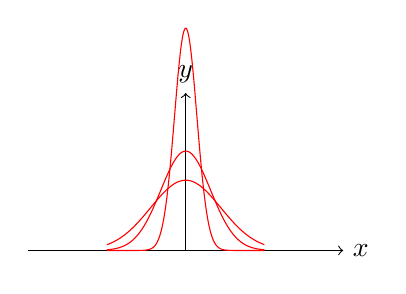
\begin{tikzpicture}
% Axes
\draw[->] (-2,0) -- (2,0) node[right] {$x$};
\draw[->] (0,0) -- (0,2) node[above] {$y$};

% Heat kernel for t = 0.1
\draw[red, domain=-1:1, samples=500] plot (\x, {1/(2*sqrt(pi * 0.1))*exp(-\x*\x/(0.1*4))});
\draw[red, domain=-1:1, samples=500] plot (\x, {1/(2*sqrt(pi * 0.05))*exp(-\x*\x/(0.05*4))});
\draw[red, domain=-1:1, samples=500] plot (\x, {1/(2*sqrt(pi * 0.01))*exp(-\x*\x/(0.01*4))});
% \draw[red, domain=-4:4, samples=100] plot (\x, {1.8*exp(-\x*\x/(0.1*4))});
\end{tikzpicture} 
  \end{center}
\end{figure}
\end{example}
\begin{proof}
 \begin{align*}
   \lim_{t \to 0+} \braket{f_t,\phi } &= \lim_{t \to 0+} \int_\mathbb{R} f_t(x) \phi(x) dx = \lim_{t \to 0+} \int_{-\infty}^{\infty} \frac{1}{2 \sqrt{\pi  t} } e^{- \frac{x^2}{4t}}  \phi(x) dx \\
                                      &= \lim_{t \to 0+} \int_{-\infty}^{\infty} \frac{1}{\sqrt{\pi }} e^{-y^2}  \phi(2ty) dy \\
                                      &\myS{*}{=} \phi(0) = \braket{\delta ,\phi }
 .\end{align*} 
 with the transformation $\frac{x}{\sqrt{2t}} = y$
\end{proof}
\begin{exercise}
 Show the change of integration and limit is valid in * 
\end{exercise}
Further examples  include : 
\begin{align*}
  Q_n(x) = \begin{cases}
    \frac{n}{2} , &\text{ if }\abs{x} \le  \frac{1}{n}\\
    0   &\text{ if } \abs{x} > \frac{1}{n} 
  \end{cases}
.\end{align*}
\begin{figure}[H]
  \begin{center}
    \begin{tikzpicture}
% Axes
\draw[->] (-2,0) -- (2,0) node[right] {$x$};
\draw[->] (0,0) -- (0,2) node[above] {$y$};

\draw[red] (-1,0)  -- (-1,1) -- (1,1) -- (1,0);
\draw[red] (-0.5,0)  -- (-0.5,2) -- (0.5,2) -- (0.5,0);
\draw[red] (-0.25,0)  -- (-0.25,3) -- (0.25,3) -- (0.25,0);
% \draw[red, domain=-4:4, samples=100] plot (\x, {1.8*exp(-\x*\x/(0.1*4))});
\end{tikzpicture} 
  \end{center}
\end{figure}
\hspace{0mm}\\
And the dirichlet kernel 
\begin{align*}
  D_n(x) = \frac{\sin(n+\frac{1}{2})x}{\sin(\frac{x}{2})} = 1+ 2\sum_{k=1}^{n}  \cos(kx)  \ \to 2\pi \delta 
.\end{align*} 
To define the notion of a distribution solving a PDE we need to first define the way we take the derivatives of distributions
\begin{definition}[Weak derivative of Distributions]
  $\forall  T \in  \mathcal{D}(\Omega )'$ . $\partial_i T$ is given by  
  \begin{align*}
    \braket{\partial_i T, \phi } \coloneqq  - \braket{T,\partial_i \phi } \quad \forall  \phi  \in \mathcal{D}(\Omega )
  .\end{align*}
  We first show this for all distributions that are defined by a $f \in L_{\text{loc}}^{1} $, every other distribution $T$ also has to satisfy this property.
\end{definition}
\begin{exercise}
  Proof the above equality for distributions $f \in  L_{\text{loc}}^{1} $ and show for arbitrary distribution $T$ that :
  \begin{align*}
    -\braket{T,\partial_i \phi }
  .\end{align*}
  is continuous and linear.\\[1ex]
  \textit{Hint : } Integration by parts; Why does it vanish on the boundary ?
\end{exercise}
\begin{example}
 For the $\delta $  distribution : 
 \begin{align*}
   \braket{\delta ^{(k)},\phi  } = (-1)^{k} \phi ^{(k)}(0)
 .\end{align*}
\end{example}
\begin{example}{Heaviside}
The Heaviside step function is defined by :
\begin{align*}
  H = \begin{cases}
    1, &\text{ if }x\ge 0 \\
    0 &\text{ if } x<0
  \end{cases} \in  L_{\text{loc}}^{1} 
.\end{align*}
\begin{align*}
  \braket{H',\phi } &\coloneqq  - \braket{H,\phi'} = - \int_{-\infty}^{\infty} H(x)\phi'(x) dx\\
                    &= - \int_0^{\infty} \phi'(x) dx = \phi(0)  =\braket{\delta,\phi }
.\end{align*}
\begin{figure}[H]
  \begin{center}
    \begin{tikzpicture}
% Axes
\draw[->] (-2,0) -- (2,0) node[right] {$x$};
\draw[->] (0,0) -- (0,2) node[above] {$y$};

\draw[red] (-2,0)  --  (0,0) -- (0,1) -- (2,1); 
% \draw[red, domain=-4:4, samples=100] plot (\x, {1.8*exp(-\x*\x/(0.1*4))});
\end{tikzpicture} 
  \end{center}
\end{figure}
\end{example}
\hspace{0mm}\\
Using all the above we can rewrite our many particle system  (MPS) by using the empiric measure and distributions 
\begin{align*}
  \begin{cases}
    \frac{d}{dt} x_i &=  \braket{K(x_i,\cdot) , \mu_N}  = \int K(x_i,y) d\mu_N(y)\\ 
    x_i(0) &= x_{i,0}
  \end{cases}
.\end{align*}
\begin{definition}[Weak Solution of MFE]
  We say $\mu $ is a weak solution of the Mean-Field-Equation (MFE) iff for $\forall  t \in  [0,T]$ , $\mu_t \in  \mathcal{M}(\mathbb{R}^{d} )$ satisfies for 
  all test functions  $\forall  \phi  \in  \mathcal{C}^{\infty}_0(\mathbb{R}^{d } )$ the following equation
  \begin{align*}
    \braket{\mu_t,\phi } - \braket{\mu_0,\phi } = \int_0^{t}  \braket{\mu_sK\mu_s,\phi } ds
  .\end{align*}
\end{definition}
\begin{remark}
  If $\mu_0 = \mu_{N,0}$  then $\mu_{N,t}$ is a weak solution of the MFE
\end{remark}
\begin{theorem}
Let the empirical measure \ref{empirical_measure} be denoted by $\mu_N$ then for "good" (regular ?)  $K(x,y)$ we have 
\begin{align*}
  \frac{d}{dt} \braket{\mu_N,\phi } = \braket{\mu_N \underbrace{\int K(x,y) d\mu_N(y)}_{=  K \mu_N}}= -\braket{\triangledown * \triangledown(\mu_N K\mu_N),\phi }
.\end{align*}
Such that $\mu_N$ is a weak solution of the MPDE
\begin{align*}
  \partial_t \mu_N + \triangledown * \triangledown(\mu_N K\mu_N) = 0
.\end{align*}  
\end{theorem}
\begin{remark}
 Note when we talk about weak solution, it means the PDE is solved in the sense of distributions.
\end{remark}
\begin{exercise}
 Show $\mu_N K \mu_N$ as defined above is a distribution for regular/ good $K(x,y)$
\end{exercise}
\begin{proof}  
\end{proof}
\begin{definition}[characteristic problem for MFE]\label{characteristic_problem}
  The corresponding characteristic is given by : 
\begin{align*}  
  \begin{cases}
    \frac{d}{dt} x(t,x_0,\mu_0) &= \int_{\mathbb{R}^{d } } K(x(t,x_0,\mu_0),y) d\mu_t(y)\\
    x(0,x_0,\mu_0) &= x_0 \in  \mathbb{R}^{d }  \\
    \mu_t &= x(t,*,\mu_0) \# \mu_0 
  \end{cases}
.\end{align*}
\end{definition}
\begin{notation}[Push Forward]
  For a measurable map $X : (\mathbb{R}^{d },\mathcal{B} ) \xrightarrow{X} (\mathbb{R}^{d },\mathcal{B} )$
  and a measure  $\mu_0 \in \mathcal{M}(\mathbb{R}^{d } )$ we have : 
 \begin{align*}
     \forall B \in  \mathcal{B} \ , \ X \# \mu_0 = \mu_0(X^{-1}(B) ) 
 .\end{align*} 
\end{notation}
\begin{exercise}
 Show that if $x(t,x_0,\mu_0) \in  \mathcal{C}^{1}(\mathbb{R},\mathbb{R}^{d } ) $  exists 
 then $\mu_t = x(t,*,\mu_0)\#\mu_0$ is a weak solution of MFE
\end{exercise}
\begin{definition}
  Space of probability measures with bounded first moment
  \begin{align*}
    \mathcal{P}_1(\mathbb{R}) \coloneqq  \{\mu_0 \in  \mathcal{M}_{+}(\mathbb{R}^{d } ) : \int_{\mathbb{R}^{d } } \abs{x} d\mu_0(x) <\infty\}  
  .\end{align*}
\end{definition}
\begin{theorem}[Uniqueness of Solution]
  For regular K (\ref{regularity})  and  $\mu_0 \in  \mathcal{P}_1(\mathbb{R}^{d } )$ then the characteristic problem \ref{characteristic_problem} has a unique solution 
  $x(t,x_0,\mu_0) \in  \mathcal{C}^{1}(\mathbb{R},\mathbb{R}^{d} ) $ and $\mu_T \in  \mathcal{P}_1(\mathbb{R}^{d} )$ , for all $t>0 $
\end{theorem}
\begin{proof}
  \textbf{Existence} \\[1ex]
 We consider 
 \begin{align*}
   x(t,x_0,\mu_0) &= x_0 + \int_0^{t} \int_{\mathbb{R}^{d } } K(x(s,x_0,\mu_0),y) d\mu_s(y) ds \\ 
                  &\myS{psh frwd.}{=} x_0 + \int_0^{t} \int_{\mathbb{R}^{d } } K(x(s,x_0,\mu_0),x(s,\zeta,\mu_0))  d\mu_0(\zeta ) ds
 .\end{align*}
% \begin{figure}[H]
%     \begin{center}
%       \begin{tikzpicture}
%         % Axes
%         \draw[] (-2,0) -- (3,0) node[right] {};
%         \draw[] (0,0) -- (0,2) node[above] {};
%         \node[left]  (0,0) {$t$};
%         \node[circle,fill,inner sep = 0.001mm] at (1,1) {$y$} ;
%         \node[left] (2,0) {$\zeta $};
%         \draw[red]  (2,0) -- (1,1);
%         \draw[red] (-2,1) --  (2,1) ; 
%   % \draw[red, domain=-4:4, samples=100] plot (\x, {1.8*exp(-\x*\x/(0.1*4))});
%   \end{tikzpicture} 
%     \end{center}
%   \end{figure}
 We define the following iteration  for all $y \in  \mathbb{R}^{d } $
 \begin{align*}
    x_0(t,y) &= y \\
    x_1(t,y) &= y + \int_0^{t} \int_{\mathbb{R}^{d}  } k(x_0(s,y),x_0(s,\zeta )) d\mu_0(\zeta ) ds \\ 
             &\vdots \\ 
    x_n(t,y) &= y + \int_0^{t} \int_{\mathbb{R}^{d}  } k(x_{n-1}(s,y),x_{n-1}(s,\zeta )) d\mu_0(\zeta ) ds \\ 
 .\end{align*}
 Similar to our proof in \label{picard1} we show the sequence is cauchy :
 \begin{align*}
   \abs{x_n(t,y) - x_{n-1}(t,y)} &\le \int_0^{t} \int_{\mathbb{R}^{d} }  \abs{K(x_{n-1}(s,y),x_{n-1}(s,\zeta )) - K(x_{n-2}(s,y),x_{n-2}(s,\zeta ))} d\mu_0(\zeta ) ds \\
                                 &\le L \int_0^{t} \int_{\mathbb{R}^{d} } \abs{x_{n-1}(s,y) - x_{n-2}(s,y)} +  \abs{x_{n-1}(s,\zeta ) - x_{n-2}(s,\zeta )} d\mu_0(\zeta ) ds\\
 .\end{align*}
 To get rid of the $\zeta $ we define  the following banach space $\mathcal{X}  = \{v \in  \mathcal{C}(\mathbb{R}^{d };\mathbb{R}^{d}  ) : \sup_x \frac{\abs{v(x)}}{1+\abs{x}} < \infty\}  $ with norm 
 \begin{align*}
   \|v\| = \sup_{x \in  \mathbb{R}^{d} } \frac{\abs{v(x)}}{1+\abs{x}}
 .\end{align*}
 We can then further approximate  by :
 \begin{align*}
   &L \int_0^{t} \int_{\mathbb{R}^{d} } \abs{x_{n-1}(s,y) - x_{n-2}(s,y)} +  \abs{x_{n-1}(s,\zeta ) - x_{n-2}(s,\zeta )} d\mu_0(\zeta ) ds \\
   &\le L \int_0^{t} \abs{x_{n-1}(s,y) - x_{n-2}(s,y)} +  \|x_{n-1}(s,* ) - x_{n-2}(s,* )\|_{\mathcal{X}} (1+C_1)  ds   
 .\end{align*}
 Where $C_1 = \int \abs{x} d\mu_0(x_0)$ is the first moment of our initial measure.
 Now we divide both sides of the inequality by $1+\abs{y}$ , and take the supremum in y 
 \begin{align*}
   \|x_n(t,*)  - x_{n-1}(t,*)\|_{\mathcal{X}} \le  L (2+C_1) \int_0^{\abs{t}} \|x_{n-1}(s,*)-x_{n-2}(s,*)\|_{\mathcal{X}}  ds
 .\end{align*}
 Then for $\forall  n > m  \gg 1$ we have 
 \begin{align*}
   \|x_{n}(t,*) - x_m(t,*)\|_{\mathcal{X}} &\le  \sum_{i=m}^{n-1} \|x_{i+1}(t,*) - x_i(t,*)\|_{\mathcal{X}} \xrightarrow{m\to \infty} 0
 .\end{align*}
 Therefore $(x_n(t,*))_{n \in  \mathbb{N}}$ is a Cauchy sequence in $\mathcal{X}$.  \\[1ex]
 Now suppose $x_n(t,*) \to x(t,*)$ : 
 \begin{align*}
   x(t,y) &= y+ \int_0^{t} \int_{\mathbb{R}^{d} }  K(x(s,y),x(s,\zeta )) d\mu_0(\zeta ) ds \\
          &= y +  \int_0^{t} \int_{\mathbb{R}^{d} }  K(x(s,y),z) d\mu_0(z) ds \\
 .\end{align*}
 This concludes the \textbf{Existence} proof \\[1ex]
 \textbf{Uniqueness : } \\[1ex]
 This proof closely mimics the one presented in \label{picard1} by using the space $\mathcal{X}$
  \end{proof}
\begin{remark}
Showing the convergence of our Picard Iteration here is slightly more complicated, forcing us to use a different norm to get a simpler
estimate to work with, remember similar trick as in functional analysis with 
\begin{align*}
  \|f\|_L = \sup_{t \in  [0,1]} e^{-Lt}\abs{f(t)} 
.\end{align*}
\end{remark}
\begin{exercise}
 Show that  $\mathcal{X}  = \{v \in  \mathcal{C}(\mathbb{R}^{d };\mathbb{R}^{d}  ) : \sup_x \frac{\abs{v(x)}}{1+\abs{x}} < \infty\}  $ with norm
 \begin{align*}
   \|v\| = \sup_{x \in  \mathbb{R}^{d} } \frac{\abs{v(x)}}{1+\abs{x}}
 .\end{align*}
 is a banach space \\[1ex]
 \textit{Hint :} Compare to supremums norm
\end{exercise}
\section{Wasserstein Distance}
\subsection{Goal}
The goal of this section is to consider  as $N \to  \infty$ how the empirical measure $\mu_{N,*}$ converges 
\begin{align*}
  \mu_{N,0} &\xrightarrow{?} \mu_0 \\
  \mu_{N,t} &\xrightarrow{?} \mu_t
.\end{align*}
we have already shown that for arbitrary given measure $\mu_0$ (on both sides of the arrows)  the PDE problem is uniquely solved,
the idea of the Mean Field Limit problem is to prove a stability result for the above convergence.
\subsection{Weak Convergence of Measure (Wasserstein Distance)}
\begin{definition}[Weak Setting of PDE problem]
 For all test functions $\phi  \in  \mathcal{C}_0^{\infty }(\mathbb{R}^{d} ) $ :
 \begin{align*}
   \int_{\mathbb{R}^{d } } \phi(x) d\mu(t,x) - \int_{\mathbb{R}^{d}} \phi(x) d\mu_0 = \int_{0}^{t} \int_{\mathbb{R}^{d} }  K\mu(s,x) \triangledown \phi(x) d\mu(s,x) 
 .\end{align*}
 Where 
 \begin{align*}
   K\mu(x) = \int_{\mathbb{R}^{d} } K(x,y) d\mu(y)
 .\end{align*}
\end{definition}
To give a small recap of what we have done so far : 
\begin{enumerate}
  \item If $\mu_{0} = \mu_{N,0} $  then $\mu_{N,t}$ is a weak solution of the above PDE 
  \item Solve the PDE for given $\mu_0 \in  \mathcal{P}_1(\mathbb{R}^{d } )$ for regular K then 
    \begin{align*}
     \mu_t = x_t \# \mu_0 
    .\end{align*}
    is a weak solution of the PDE
\end{enumerate}
The next goal is to consider the problem  
\begin{align*}
  \text{if } \mu_{N,0} \to \mu_0 \quad \text{ then } \mu_{N,t} \to \mu_t
.\end{align*}
$\Leftrightarrow$ stability of PDE
\begin{definition}[Wasserstein Distance]
  For all $\mu , \nu  \in  \mathcal{P}_p(\mathbb{R}^{d} )$  , $(p\ge 1) $ the Wasserstein Distance of $\mu $ and $\nu $ is given by 
  \begin{align*}
    W^{p}(\mu ,\nu ) = \dist_{MK,p}(\mu ,\nu ) = \inf_{\pi \in  \Pi(\mu ,\nu )} \left( \int \int_{\mathbb{R}^{2d} } \abs{x-y}^{p} \pi(dxdy) \right)^{\frac{1}{p}}  
  .\end{align*}
  Where  
  \begin{align*}
    \Pi(\mu ,\nu ) = \{\pi \in \mathcal{P}(\mathbb{R}^{d} \times  \mathbb{R}^{d}  ) : &\int_{\mathbb{R}^{d}\times E } \pi(dx,dy) = \nu(E) \\
                                                                                      &\int_{E \times  \mathbb{R}^{d} } \pi(dx,dy) = \mu(E)\}  
  .\end{align*}
\end{definition}
\begin{exercise}
 For two deterministic measures $\delta_x,\delta_y$ prove 
 \begin{align*}
  W^{1}(\delta_x,\delta_y)  = \abs{x - y}
 .\end{align*}
\end{exercise}
\begin{remark}
 If $\phi , \psi \in  \mathcal{C}(\mathbb{R}^{d} )$  s.t :
 \begin{align*}
   \phi(x) &\sim  \abs{x}^{p}  \quad \forall \ \abs{x} \gg 1 \\
   \psi(x) &\sim  \abs{y}^{p}  \quad \forall \ \abs{y} gg 1
 .\end{align*}
 Then 
 \begin{align*}
   \int \int_{\mathbb{R}^{2d} } (\phi(x) + \psi(y)) \pi(dx,dy) = \int_{\mathbb{R}^{d } } \phi(x) d\mu(x) + \int_{\mathbb{R}^{d} } \psi(y) d\nu(y)
 . \end{align*}
\end{remark}
\begin{corollary}[Kontonovich-Rubinstein duality]
 \begin{align*}
   \dist_{MK,1}(\mu ,\nu ) &= W^{1}(\mu ,\nu )  \\
                           &= \sup_{\phi \in  \text{Lip}(\mathbb{R}^{d} )} \abs{\int_{\mathbb{R}^{d} } \phi(x) d\mu(x) - \int_{\mathbb{R}^{d} } \phi(x) d\nu(x)}
 .\end{align*} 
 $\text{Lip}(\phi ) = 1$
\end{corollary}
The proof of the above can be found in the book xyz
\begin{theorem}[Dobrushin's stability]
  Let $\mu_{0},\overline{\mu }_0  \in  \mathcal{P}_1(\mathbb{R}^{d } )$\\
  Then let $(x(t,*,\mu_0),\mu_t(*)),(x(t,*,\overline{\mu }_0 ),\overline{\mu }_t(*) )$ be solutions of 
  the corresponding PDE problem. For arbitrary $\forall\ t >0$ it holds that the distance 
  \begin{align*}
    \dist_{MK,1}(\mu_t,\overline{\mu }_t ) \le e^{2\abs{t}L} \dist_{MK,1}(\mu_0,\overline{\mu }_0 )
  .\end{align*} 
\end{theorem}
\begin{proof}
  For initial data $\mu_{0} ,\overline{\mu}_0$ we want to compare the trajectories
 \begin{align*}
   x(t,x_{0},\mu_{0}) - x(t,\overline{x}_0,\overline{\mu }_0 ) = x_{0}-\overline{x}_0 &+ \int_0^{t} \int_{\mathbb{R}^{d } } K(x(s,x_{0},\mu 0),x(s,z,\mu_0))   d\mu_0(z) ds \\
                                                                                      &- \int_0^{t} \int_{\mathbb{R}^{d} } K(x(s,\overline{x}_0,\overline{\mu }_0  ),x(s,\overline{z },\overline{\mu }_0  )) d\overline{\mu}_0(\overline{z} ) ds
 .\end{align*}
 We need to combine the above two integrals together, while the time integrals are the same, but the space integral has to be converted into 2d dimensions by inserting $1 = \int_{\mathbb{R}^{d} } d\mu_0(z)$
 \begin{align*}
   x(t,x_{0},\mu_{0}) - x(t,\overline{x}_0,\overline{\mu }_0 ) + \int_0^{t} &\iint   K(x(s,x_{0},\mu 0),x(s,z,\mu_0)) \\
   &- K(x(s,\overline{x}_0,\overline{\mu }_0  ),x(s,\overline{z },\overline{\mu }_0 ))  d(\mu_0 \times \overline{\mu }_0)(z,\overline{z} ) ds
 .\end{align*}
 Let $\pi_0 \in  \Pi(\mu_{0},\overline{\mu }_0 )$ then we can estimate point-wise for fixed $x_{0},\overline{x }_0 $:
 \begin{align*}
   \|x(t,x_{0},\mu_0) - x(t,\overline{x}_0,\overline{\mu }_0  )\| \le  \|x_{0}-\overline{x}_0 \| + L\int_0^{t} &\iint_{\mathbb{R}^{2d } } \|x(s,x_{0},\mu_0) - x(s,\overline{x }_0,\overline{\mu }_0  )\| \\
                                                                                                                                       &+ \|x(s,z,\mu_0) - x(s,\overline{z},\overline{\mu }_0  )\| d\pi_0(z,\overline{z} ) ds
 .\end{align*}
 Now taking the integral on both sides : 
 \begin{align*}
   \iint_{\mathbb{R}^{2d } }  \|x(t,x_{0},\mu_0) - x(t,\overline{x}_0,\overline{\mu }_0  )\| d\pi_0(x_{0},\overline{x}_0 ) &\le \iint_{\mathbb{R}^{2d} } \|x_{0}-\overline{x}_0 \| d\pi_0(x_{0},\overline{x}_0 ) \\
                                                                                                                               &+ L\int_0^{t}  \iint_{\mathbb{R}^{2d } }  \|x(s,x_{0},\mu_0) - x(s,\overline{x }_0,\overline{\mu }_0  )\| d\pi_0(z,\overline{z} ) ds \\
                                                                                                                               &+   L \int_0^{t} \int \int_{\mathbb{R}^{2d} }  \|x(s,z,\mu_0) - x(s,\overline{z},\overline{\mu }_0  )\| d\pi_0(z,\overline{z} ) d\pi_0(z,\overline{z}) ds
 .\end{align*}
 Now we define : 
 \begin{align*}
   D[\pi_0](t) = \int \int_{\mathbb{R}^{d} } \|x(s,z,\mu_0) - x(s,\overline{z},\overline{\mu }_0  )\| d\pi_0(z,\overline{z} )
 .\end{align*}
 We obtain that the distance based on the measure $\pi_0$ at time t :
 \begin{align*}
   D[\pi_0](t) \le  D[\pi_{0}](0) + 2L \int_0^{t} D[\pi_0](s) ds
 .\end{align*}
 We can now use  Gronwalls inequality 
 \begin{align*}
   D[\pi_0](t) \le D[\pi_0](0)*e^{2L\abs{t}}
 .\end{align*}
 Where the above inequality holds for arbitrary $ \pi_0 \in  \Pi(\mu_{0},\overline{\mu }_0 )$
 \begin{align*}
   \inf_{\pi_0 \in  \Pi(\mu_0,\overline{\mu }_0 )} D[\pi_0](t) \le \inf_{\pi_0 \in  \Pi (\mu_0,\overline{\mu }_0 )} D[\pi_0](0)*e^{2Lt}  = \dist_{MK,1}
 .\end{align*}
 Now all we need to show is that 
 \begin{align*}
   \dist_{MK,1} = \inf_{\pi_0 \in  \Pi(\mu_0,\overline{\mu }_0 )} D[\pi_0](t)  = \inf_{\pi_t \in  \Pi(\mu_t,\overline{\mu }_t )} \int \int \abs{x-\overline{x} } d\pi_t(x,\overline{x} )
 .\end{align*}
 It remains to be prove that for
 \begin{align*}
  \phi_t(x_{0},\overline{x}_0 ) = (x(t,x_{0},\mu_{0}),x(t,\overline{x}_0,\overline{\mu }_0  ))
 .\end{align*}
 the push forward measure $\phi_t \# \pi_0 \in  \Pi(\mu_t,\overline{\mu }_t )$ for $\forall  \ \pi_0 \in  \Pi(\mu ,\overline{\mu }_0 )$
\end{proof}
\begin{exercise}
  Prove that for arbitrary $\pi_0 \in  \Pi(\mu_0,\overline{\mu }_0 )$  the push forward measure $\phi_t \# \pi_0 \exists  \Pi(\mu_t,\overline{\mu }_t )$ for 
  \begin{align*}
    \phi_t(x_{0},\overline{x}_0 ) : \mathbb{R}^{2d} \to  \mathbb{R}^{2d} \ \phi_t(x_{0},\overline{x}_0 )   = (x(t,x_{0},\mu_0),x(t,\overline{x}_{0},\overline{\mu}_0))
  .\end{align*}
\end{exercise}
We are also interested in what happpens when the initial data is good
\begin{corollary}
 If $\mu_{0}$  has a density  $f_{0} \in  L^{1}(\mathbb{R}^{d} ) $a with finite first moment : 
 \begin{align*}
   \int_{\mathbb{R}^{d} } \abs{x} f_{0}(x) dx < \infty
 .\end{align*}
 Then the Cauchy problem 
 \begin{align*}
   \partial_t f  + \triangledown * (fkf) &= 0  \\
   f_0 \vert_{t=0} = f_{0}
 .\end{align*}
 has a unique weak solution $f \in  \mathcal{C}(\mathbb{R};L^{1}(\mathbb{R}^{d} ) )$ i.e $\forall \ \phi  \in  \mathcal{C}_0^{\infty}(\mathbb{R}^{d} ) $ it holds : 
 \begin{align*}
   \int_{\mathbb{R}^{d} }\phi(x) f(x,t) dx - \int_{\mathbb{R}^{d} }\phi(x) f_0(x) dx = \int_0^{t} \int_{\mathbb{R}^{d} } f(x,t)Kf(x,t) \triangledown \phi(x) dx ds
 .\end{align*}
 and  for all $t \in  \mathbb{R}$
 \begin{align*}
   \|f(*,t)\|_{L^{1}(\mathbb{R}^{d} ) } \in  \mathcal{C}(\mathbb{R})
 .\end{align*}
\end{corollary}
\begin{proof}
  Left as an exercise
\end{proof}
\begin{exercise}
We already know the weak-solution $\mu_t$  exists such that it remains to show that for $\forall \ t \in  \mathbb{R}$ , $\mu_t \in  \mathcal{P}_1(\mathbb{R}^{d} )$ is absolute continuous 
with respect to the Lebesgue measure, prove this statement
\end{exercise}
\begin{theorem}[mean field limit ]
  For arbitrary initial data $\forall \ f_{0} \in  L^{1}(\mathbb{R}^{d} ) $ , let $\mu_{N,0} = \frac{1}{n} \sum_{i=1 }^{N} \delta_{x_{i,0}} $
  s.t the distance 
  \begin{align*}
    \dist_{MK,1}(\mu_{N,0},f_{0}) \xrightarrow{N \to \infty} )
  .\end{align*}
  and $x_N(t)$ be the solution of many particle system wiht ID $x_{i,0}$ then 
  the corresponding empirical measure $\mu_{N,t} = \frac{1}{N} \sum_{i=1 }^{N} x_{i}(t) $ it holds : 
  \begin{align*}
    \dist_{MK,1}(\mu_{N,t},f_t) \le  e^{2Lt} \dist_{MK,1}(\mu_{N,0},f_{0}) 
  .\end{align*}
  Where $f_t$ is the corresponding density resulting from the previous corollary of the PDE weak solution.\\[1ex]
  and furthermore $\mu_{N,t} \xrightarrow{N\to \infty} f(*,t)$ weakly in measure i.e 
  \begin{align*}
    \forall  \phi \in \mathcal{C}_b(\mathbb{R}^{d } ) \ : \ \int \phi  d\mu_{N,t} \to  \int \phi(x) f_t(x) dx
  .\end{align*}
\end{theorem}
\begin{exercise}
  Find a sequence of empirical measures that converges against a density.
\end{exercise}

% http://www.cmls.polytechnique.fr/perso/golse/M2/PolyKinetic.pdf
